\documentclass[english, a4paper, 12pt, twoside]{article}

% -----------------------------

%
% config
%
% -----------------------------
%
% user dependent configuration
%

% enter your personal information:
\newcommand{\authorname}{Juan Jose Arango Serrano}
\newcommand{\authorid}{1861694}
\newcommand{\authormail}{s2juaran@uni-trier.de}
\newcommand{\authoraddress}{
}
% course of study
\newcommand{\courseofstudy}{Your Course of Study}

% enter your works title:
\newcommand{\thesistitle}{
    Your Thesis Title
}

% course information
\newcommand{\moduletitle}{Module Title}
\newcommand{\moduleid}{XXXXXXXX}


% enter start and submission date:
%\newcommand{\submissiondate}{\today}

% enter first (and second) supervisor name:
%\newcommand{\supervisor}{Prof. Dr. Supervisor}

% enter your references path:
\newcommand{\references}{references.bib}

% -----------------------------

% -----------------------------

%
% preamble
%
\usepackage{./cldh/preamble}
\usepackage[utf8]{inputenc}
\usepackage[T1]{fontenc}
% -----------------------------

\begin{document}

% -----------------------------
%

\fancypagestyle{frontpage}{
	\fancyhf{}
	\renewcommand{\headrulewidth}{0pt}
	\renewcommand{\footrulewidth}{0pt}
	\vspace*{1\baselineskip}
	
    \fancyhead[L]{ 
\includegraphics[width=6cm]{./cldh/university_logo.png}}
	\fancyhead[R]{
        Universität Trier, Fachbereich II \\ 
        Professur Computerlinguistik
    }
    \setlength{\headheight}{56pt}
}

\begin{titlepage}
	
    \newgeometry{top=1 in, bottom=2 in, left=1 in, right= 1 in} 
    \thispagestyle{frontpage}

    \begin{center}
        
        \vspace*{6\baselineskip}
        
        {\Large \textbf{\thesistitle}} \\
        
        \vspace*{1.5\baselineskip}

        {\large \moduletitle \ (\moduleid)} \\
        {\large \courseofstudy} \\

        \vfill

        \large{submitted by} \\
        \vspace{0.8\baselineskip}

        % Three Authors in a clean table
        {\large
        \begin{tabular}{c c c}
            \textbf{\authorone} & \textbf{\authortwo} & \textbf{\authorthree} \\
            \small Matr. \authoridone & \small Matr. \authoridtwo & \small Matr. \authoridthree \\
            \small \authoremailone & \small \authoremailtwo & \small \authoremailthree \\
        \end{tabular}
        }

        \vfill        

        % Instructor and Date at the bottom
        \begin{tabular}{r l}
            \textbf{Instructor:} & \supervisor \\
            % \textbf{Date:} & \today
        \end{tabular}

    \end{center}

    
\end{titlepage}
\restoregeometry % Returns margins to normal for the rest of the doc

% -----------------------------
%
%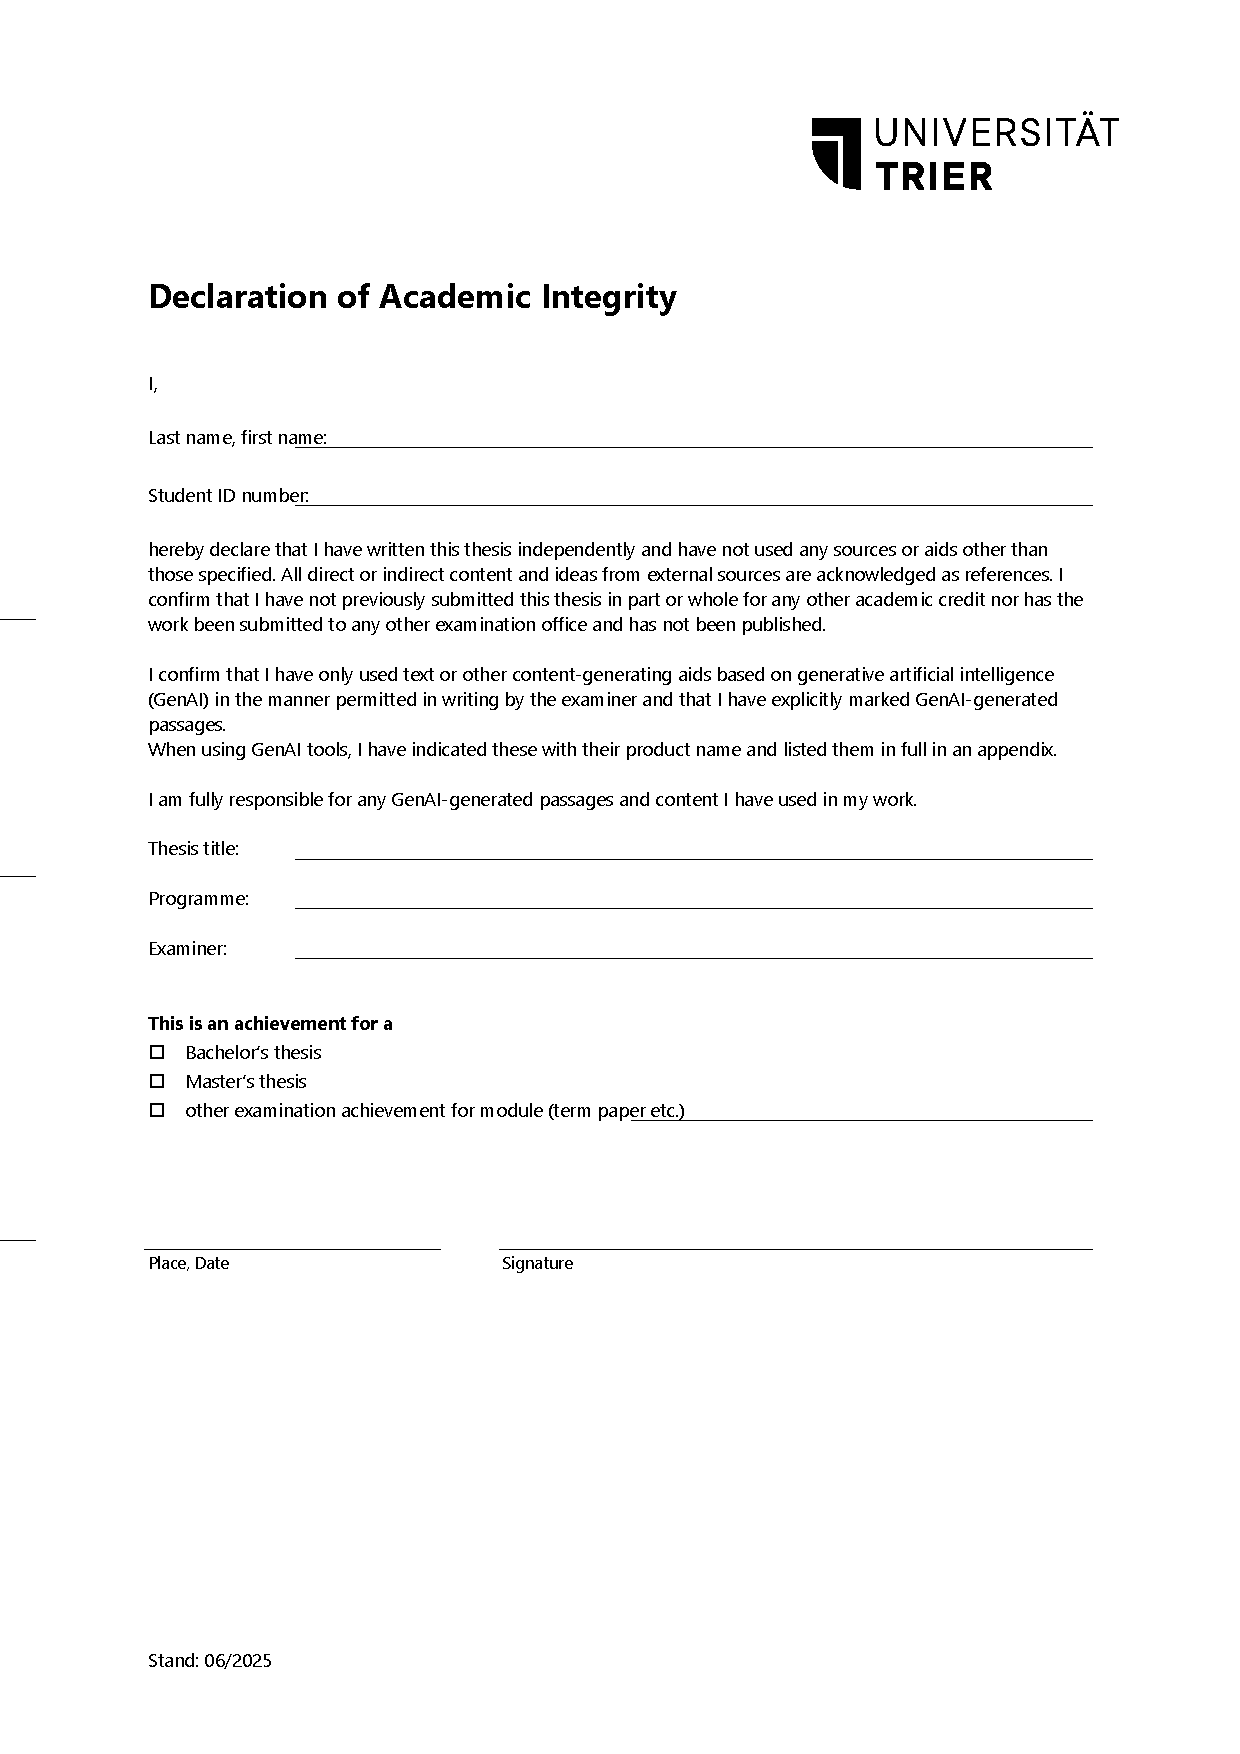
\includepdf[pages=-]{./cldh/Eigenstaendigkeitserklaerung_Englisch.pdf}
\newpage

%\tableofcontents
\newpage

% -----------------------------
% -----------------------------
% BEGIN 
\pagenumbering{arabic} %all styles: arabic, alph, Alph, roman or Roman

\begin{abstract}
Multilingual foundation models represent a central trend in modern machine learning, yet pretraining across massive corpora often encodes social biases. While previous studies have demonstrated that static embeddings distilled from contextualized models encode gender bias in English, Spanish presents a particular challenge as most professions are morphologically gender marked, confusing grammatical gender with social bias. 

This study evaluates how static embeddings extracted from multilingual models assign gender bias to grammatically invariant Spanish professions (e.g., \textit{dentista}, \textit{taxista}) without explicit supervision. Comparative analysis is conducted
across Arabic and Tigrina. 

Using geometric test across multiple architectures, we demonstrate that while models successfully encode the grammatical neutrality of certain suffixes, statistical frequency and societal bias override morphological rules for fields historically dominated by men. Finally, our results demonstrate that the internal design of the model also has an influence bias direction. 


\end{abstract}

\section{Introduction}\label{section-introduction}
Large language models trained across numerous languages represent a central trend in modern machine learning. Models such as mBERT and the XLM RoBERTa family create shared representational spaces for dozens of languages. This compression raises an important structural question, when languages with radically unequal training data coexist, how do these models distribute social associations across them? \textcite{Bommasani:2020} demonstrated that static embeddings distilled from English contextualized models encode social biases. However, English nouns generally lack grammatical gender. In Spanish, is very common to find nouns marked by gender (e.g., \textit{maestro/maestra}), which often confuses grammatical gender with social bias.

This research investigates how these models handle grammatically neutral Spanish professions compared to those with explicit gender markers. We also place Spanish within a broader comparative context alongside languages with lower training resources, such as Tigrinya and Arabic. By examining these models across their entire depth, we aim to understand how gender bias varies from the initial input to the final output. Previous studies establish that early layers process syntax while middle layers encode semantic relationships, which is exactly where we expect social associations to peak before a final representational collapse at the output layer.

Furthermore, we evaluate the robustness of our geometric bias measurements. We test whether a projection estimator sensitive to magnitude and a cosine estimator based entirely on angles agree on the underlying trends. We observed a Spearman correlation exceeding 0.96 across all valid models, confirming the reliability of our mathematical approach.

This research aims to fill the identified gap with a layer wise, cross linguistic and architecture comparative, with Spanish as the main focus, following the questions:
\begin{itemize}
    \item \textbf{RQ1}: Do multilingual transformers encode measurable gender bias in Tigrigna, Arabic, and Spanish under a unified geometric protocol?
    \item \textbf{RQ2}: How does measured bias vary across transformer layers, and at which depths do associations peak?
    \item \textbf{RQ3}: Do two independent geometric estimators agree on bias trends across models?
    \item \textbf{RQ4}: Does attention architecture determine gender bias direction, independent of pretraining data?
\end{itemize}

\section{Related Work}\label{section-methodology}
\subsection{Bias in Static Word Embeddings}
Early work established that social biases are encoded geometrically in static word embeddings. \textcite{Bolukbasi:2016} derived a gender direction from anchor sets, revealing systematic profession gender associations and proposing projection based debiasing. \textcite{Caliskan:2017} introduced WEAT as a statistical
framework for implicit associations; \textcite{Garg:2018}  showed embedding bias correlates with historical
trends. \textcite{Gonen:2019} demonstrated that removing a single bias direction does not eliminate
deeper geometric bias, motivating continued geometric analysis.

\subsection{Interpreting Contextual Representations via Reductions}
Transformer models produce contextualised representations that vary across inputs and depth, complicating direct application of geometric methods. \textcite{Bommasani:2020} formalised reductions of contextual embeddings to stable word level vectors suitable for geometric analysis, while \textcite{Rogers:2020} surveys the unequal distribution of linguistic information across transformer layers, motivating layer wise analysis.

\subsection{Multilingual Bias and Cross-Lingual Considerations}
As multilingual transformers became widely adopted, bias analysis extended beyond English. \textcite{Zhao:2019} and \textcite{Zhao:2020} showed that geometric bias methods transfer to contextual multilingual models and that bias patterns vary substantially across languages, with debiasing in one language not generalising to others. \textcite{Guo:2021} further showed contextualised embeddings encode intersectional associations. These studies predominantly evaluate final layer representations. \textcite{Lauscher:2020}
showed zero shot cross lingual transfer degrades substantially for typologically distant and low resource languages. 


\subsection{Architecture-Driven Effects on Representations}
The models evaluated here differ not only in scale but in fundamental attention design. \textcite{He:2021} introduced Disentangled Attention, which separates content and positional information into independent attention matrices, substantially changing how contextual relationships are encoded across layers. \textcite{He:2023} extended this design to multilingual pretraining via an ELECTRA-style training objective, producing the microsoft/mdeberta-v3-base checkpoint evaluated here. \textcite{Liang:2023} enlarged the Sentence Piece vocabulary from 250K tokens (XLM-R) to 1M tokens (XLM-V) to improve tokenisation coverage for
low resource languages. These architectural and vocabulary decisions constitute the design space whose bias consequences this study directly compares.

\subsection{How This Work Differs}
We integrate geometric bias analysis  \textcite{Bolukbasi:2016} with contextual-to-static reductions \textcite{Bommasani:2020} in a controlled layer wise, architecture comparative study across five multilingual models, revealing that Disentangled Attention produces a complete reversal of gender bias direction not previously documented in the multilingual bias literature.


\section{Methodology}\label{section-methodology}

\subsection{Models}
We evaluate four pretrained multilingual transformer models without fine tuning. All checkpoints are loaded from HuggingFace Hub; no parameter updates are performed.
\begin{itemize}
    \item \textbf{mBERT} (\texttt{bert-base-multilingual-cased}; \cite{Devlin:2019}): 
    A 12-layer Transformer model (yielding 13 hidden states including the embedding layer). It employs a WordPiece vocabulary of approximately 120K tokens covering 104 languages. It serves as our baseline for multilingual pre-training.

    \item \textbf{XLM-RoBERTa-base} (\texttt{xlm-roberta-base}; \cite{Conneau:2020}): 
    Consists of 12 layers (13 hidden states) with a 250K-token SentencePiece vocabulary. It was trained on 2.5TB of CommonCrawl data, significantly scaling the training data compared to mBERT.

    \item \textbf{XLM-RoBERTa-large} (\texttt{xlm-roberta-large}; \cite{Conneau:2020}): 
    A larger variant featuring 24 layers (25 hidden states) and a hidden dimension of 1024. It utilizes the same 250K SentencePiece vocabulary as the base model but provides higher capacity for complex linguistic patterns.

    \item \textbf{XLM-V-base} (\texttt{facebook/xlm-v-base}; \cite{Liang:2023}): 
    This model maintains a 12-layer architecture (13 hidden states) but features an expanded SentencePiece vocabulary of 1M tokens. This design choice aims to solve the "vocabulary bottleneck" observed in low-resource language processing.

    \item \textbf{mDeBERTa-v3-base} (\texttt{microsoft/mdeberta-v3-base}; \cite{He:2023}): 
    Comprising 12 layers (13 hidden states), this model utilizes \textit{Disentangled Attention}. Unlike the standard Transformer architecture which sums content and position embeddings, DeBERTa represents them separately. The attention weight $A_{i,j}$ between token $i$ and $j$ is calculated as:

\end{itemize}

\subsection{Languages and Data}

This study focuses on Spanish (\textit{es}). We utilize a sentence level corpus derived from \textbf{Spanish Wikimedia}, containing 100,000 sentences to provide a broad representation of natural language patterns.

\textbf{Gender Anchors:} To define the semantic gender direction, we employ a set of definitional anchor pairs (e.g., \textit{él/ella}, \textit{hombre/mujer}). These pairs provide the reference points for calculating the gender subspace in the embedding layers \parencite{Bolukbasi:2016, Zhao:2019}.

\textbf{Profession Lists:} To isolate morphosyntactic properties from latent societal bias, we organize two distinct target lists of profession terms:
\begin{itemize}
    \item \textbf{Group A (Invariant):} Grammatically neutral terms that remain identical regardless of the referent's gender (e.g., \textit{dentista}, \textit{comerciante}, \textit{estudiante}, \textit{periodista}). 
    \item \textbf{Group B (Marked):} Grammatically gendered terms that possess distinct masculine and feminine forms (e.g., \textit{ingeniero/ingeniera}, \textit{abogado/abogada}). These serve as a baseline to establish the expected magnitude of the gender signal when it is explicitly encoded in the surface form.
\end{itemize}

\subsection{Context Sampling}
For each target word \textit{w}, we retrieve up to n sentences containing w via substring matching. We use \textit{n} = 20
contexts per profession term and \textit{n} = 12 contexts per anchor term across all languages, to ensure stable cen-
troid estimation within CPU memory constraints. Words with fewer than the minimum available contexts
are excluded.


\subsection{Contextual to Static Reduction}
Transformer models produce contextualised token representations that vary across inputs. To enable geometric analysis, we adopt the reduction framework of \cite{Bommasani:2020}. For each occurrence of word $w$ in context $c_i$, subword representations are mean-pooled. The result is averaged across $n$ contexts. Formally, at layer $\ell$:
\begin{equation}
\label{eq:reduction}
s_\ell(w) = \frac{1}{n}\sum_{i=1}^n h_\ell(w, c_i),
\end{equation}
where $h_\ell(w, c_i)$ is the mean pooled subword representation. This yields one stable static embedding per layer for each target word.

\subsection{Gender Direction Construction}
Following \cite{Bolukbasi:2016}, we define a gender direction using predefined anchor sets. Let $M$ and $F$ denote the male and female anchor term sets. For each layer $\ell$, anchor representations are reduced following Eq. \eqref{eq:reduction}, and the centroids for the male and female anchor sets ($A_M$ and $A_F$) are defined as: 
\begin{equation}
c_{M,\ell} = \frac{1}{|M|}\sum_{w \in M} s_\ell(w), \quad c_{F,\ell} = \frac{1}{|F|}\sum_{w \in F} s_\ell(w),
\end{equation}
and the layer specific gender direction is:

\begin{equation}
g_\ell = c_{M,\ell} - c_{F,\ell}.
\end{equation}

This vector encodes the principal geometric contrast between male and female anchors at layer $\ell$ \parencite{Bolukbasi:2016}.

\subsection{Bias Measurement and Agreement}
For each profession $p$ and layer $\ell$ we compute two geometric estimators:
\begin{enumerate}[(a)]
    \item \textbf{Gender Direction Projection (\texttt{proj})}: The scalar projection of $s_\ell(p)$ onto the gender direction:
    \begin{equation}
    ProjBias_\ell(p) = \frac{s_\ell(p) \cdot g_\ell}{\|g_\ell\|}.
    \end{equation}
    Positive values indicate alignment toward the male centroid; negative values indicate alignment toward the
female centroid. The scalar projection preserves vector magnitude and is sensitive to the strength of the
gender association \parencite{Bolukbasi:2016}.
    \item \noindent \textbf{Centroid Cosine Difference (\texttt{cosdiff})}. As a complementary magnitude normalised estimator:

\begin{equation}
    \text{CosBias}_\ell(p) = \cos(\mathbf{s}_\ell(p), \mathbf{c}_{M,\ell}) - \cos(\mathbf{s}_\ell(p), \mathbf{c}_{F,\ell}),
\end{equation}

where cosine similarity is defined as \parencite{Manning:2008}:

\begin{equation}
    \cos(\mathbf{a}, \mathbf{b}) = \frac{\mathbf{a} \cdot \mathbf{b}}{\|\mathbf{a}\| \|\mathbf{b}\|} .
\end{equation}
\end{enumerate}


This estimator directly compares relative angular proximity to male and female centroids and is invariant
to vector scale.


\subsection{Estimator Agreement}
To assess measurement robustness, we compute Spearman rank correlation \parencite{Spearman:1904} between the two estimators across profession terms at each layer:
\begin{equation}
\rho_\ell = \text{Spearman}(\{ProjBias_\ell(p)\}_p, \{CosBias_\ell(p)\}_p).
\end{equation}

$\rho\ell$ = 1 indicates perfect ordinal agreement across professions.

\subsection{Layer-Wise Aggregation}
For visualisation we compute the mean projection score across retained profession terms at each layer $\ell$,
yielding a layer-wise bias trajectory:

\begin{equation}
    \overline{\text{Proj}}_\ell = \frac{1}{|P|} \sum_{p \in P} \text{ProjBias}_\ell(p),
\end{equation}

where \textit{P} is the set of retained professions. This trajectory summarises how the overall geometric gender
signal evolves across model depth.


\section{Results}\label{section-results}
The experimental results show that gender bias is a real and measurable feature in the models in this study. We first verified if our measurement methods were reliable by checking if the two different scoring techniques produced the same results. Over every model, we found nearly perfect agreement in the middle layers, with correlation values staying above 0.99. This high level of consistency proves that the math is picking up on genuine patterns in the word vectors and that the findings are not simply the result of random errors.

For the neutral professions in Group A, many terms like dentista and estudiante stayed close to the neutral mark of zero. However, the data for comerciante (merchant) showed that bias can vary significantly depending on the models' architecture. While mDeBERTa-v3-base correctly identified this word as neutral with a score of -0.0310, xlm-v-base assigned it a strong male score of +1.9509. The XLM-RoBERTa models were in between these values.

Regarding the gendered pairs in Group B, Masculine professions like abogado and ingeniero showed strong positive values in the projection scores, whereas their feminine counterparts, such as abogada and ingeniera, consistently show negative scores indicating their belonging to the female side. However, there is a significant asymmetry in magnitude. While masculine terms are located very far from the center, the feminine terms stay much closer to the neutral center despite their female leaning.

The layer-wise projection curve demonstrates that the bias signal is not constant across the network. It is weakest in the first layers, reaches its peak intensity in the middle layers (typically between layers 6 and 9), and decreases slightly toward the output layers. It is a pattern that shows how the model builds these gender associations as it processes the input through its internal layers, reaching a maximum point before preparing the final representation.

\section{Conclusions}\label{section-conclusions}
The findings of this study show that language models have the ability to learn the grammatical
rules of neutral Spanish nouns without direct supervision. For instance, professions
with -ista or -ante suffixes (e.g., dentista, artista, estudiante, and cantante) are
consistently clustered near the origin (projection scores close to zero). 


However, the results also highlight a conflict between these linguistic rules and societal frequency. When a profession is historically associated with men in the real world, the statistical bias in the training text often overrides the grammar. This explains why a word like \textit{comerciante} appears heavily biased in certain models despite being grammatically neutral. The better performance of \texttt{mDeBERTa-v3-base} in these cases suggests that certain model designs, particularly those with different attention mechanisms, might be more effective at keeping grammar and social stereotypes separate.

Finally, the data show that the Spanish masculine generic creates a "masculine default" within the vector space. Because masculine forms appear much more frequently and in more varied contexts, the models treat them as the standard representation and treat feminine forms as secondary variations. This can be seen by the fact that feminine terms stay closer to the neutral origin than masculine terms do. This indicates that even though the models acknowledge the feminine gender, the masculine form acts as the primary geometric anchor for the concept of the profession itself. Consequently, as long as models learn from human generated text, the heavy influence of social bias will likely keep prioritizing deep rooted stereotypes over the strict grammatical rules.


All experiments are implemented in Python and the full pipeline is publicly available at https://github.com/HDGeeks/ML4NLU-PAPER.


% END
% -----------------------------
% -----------------------------

%
% references
%
\newpage
\printbibliography

\end{document}